%\documentclass[12pt,draft]{article}
\documentclass[12pt]{article}
\usepackage{CJK}
\usepackage{mathrsfs}
\usepackage{amsmath,amsthm,amsfonts,amssymb}
\usepackage{geometry}
\usepackage{fancyhdr}
\usepackage{indentfirst}
\usepackage{float}
\usepackage[dvips]{graphicx}
\usepackage{subfigure}
\usepackage[font=small]{caption}
\usepackage{threeparttable}
\usepackage{cases}
\usepackage{multicol}
\usepackage{url}
\usepackage{amsmath}
\usepackage{bm}
\usepackage{xcolor}
\usepackage{overpic}
\usepackage[round]{natbib}
\usepackage[utf8]{inputenc}
\usepackage[american]{babel}
\usepackage{graphicx}
\numberwithin{equation}{section}
\geometry{left=1.5cm,right=1.5cm,top=1.5cm,bottom=1.5cm}
\setlength{\parskip}{0.3\baselineskip}
\setlength{\headheight}{15pt}
\usepackage{color}   %May be necessary if you want to color links
\usepackage{hyperref}
\hypersetup{
    colorlinks=true, %set true if you want colored links
    linktoc=all,     %set to all if you want both sections and subsections linked
    linkcolor=blue,  %choose some color if you want links to stand out
}
\begin{document}\small
\title{ING3 Report}
\author{Yan JIN}
\pagestyle{fancy}\fancyhf{}
\lhead{}\rhead{JIN Yan}
\lfoot{\textit{}}\cfoot{}\rfoot{\thepage}
\renewcommand{\headrulewidth}{1.pt}
\renewcommand{\footrulewidth}{1.pt}
\maketitle
\tableofcontents
%=======================================
\section{Introduction to Question-Answering System}
	In 2011, IBM's Watson question-answering system won the TV game show Jeopardy! against all the humans, that surprised all the world. And the famous already in use applications like Siri, Google Search etc. are also the results of the question-answering systems.  \par
\subsection{Factoid questions}
	QA is an AI-complete problem, implying that if we solve QA, we will solve all the other problems too. But the systems now mainly focus on \textbf{factoid questions}, which can be answered with simple facts expressed in short text answers. \par
%--------------------------------------------
\subsection{Knowledge bases}
	Lots of recent developments in Question-answering system is based on knowledge bases(KBs)\citep{unger2014introduction}. Knowledge bases typically represent their data as triples like: (president-of, Trump, United States). Freebase and Dbpedia are two large typical knowledge bases.\par
%=======================================
\subsection{Areas in  Question-Answering System}
	There are several areas in Question answering:
	\begin{enumerate}
	\item Semantic Parsing\par
		Semantic Parsing focus on constructing a semantic parser that could convert natural language questions into structured expressions like logical forms. And it can be used to query a knowledge base.\par
		Context is a Knowledge base, and the answer is a logical form. \par
	\item Information retrieval \par
		Information retrieval directly search answers from a corpus of documents based on the information conveyed in questions. \par
		Context is a corpus of documents, and the answer is a document, a paragraph or a sentence.
	\item Reading Comprehension\par
		Context is a specific document, and the answer is based on that specific document given.
	\item Visual QA \par
		Context is a one or several images, and the answer is simple facts.
	\end{enumerate} \par
	This article focus on the recent neural network approach to some of these areas. \par
%=======================================
\subsection{Neural network-based methods for Question-Answering System}
	The first NN-based methods is introduced by Antoine Bordes in 2014\citep{bordes2014open}, which represent both the questions and answers as semantic vectors, so that no needs for pre-defined grammars or lexicons by hand. This approach is based on learning low-dimensional vector embeddings of words. \par
	Let K denotes the knowledge bases, and {\it q} denotes a question, {\it a} a candidate answer. The model is to learning a score function, which gives the best answer $\hat{a}$ for the question {\it q}: 
	\begin{equation}
		\hat{a} = argmax_{a \in K} S(q, a)
	\end{equation}
where the score function is:
	\begin{equation}
		S(q,a) = f(q)^T g(a)
	\end{equation} 
where $f(\cdot)$ is a function mapping words from question into $\mathbb{R}^k$; $g(\cdot)$ is a function mapping entities and relationships from KB triples into $\mathbb{R}^k$. \par 
	From his later paper in the same year\citep{bordes2014question}, he made a simple changement and improved this model to achieve a better result than all the other traditional methods. The key idea was with the help of the concept of subgraph embedding, adding more information in the answer end.\par
	In 2015, the score function is improved into three parts\citep{dong2015question}:
	\begin{equation}
		S(q,a) = \underbrace{f_1(q)^T g_1(a)}_{\text{answer path}} + \underbrace{f_2(q)^T g_2(a)}_{\text{answer context}}  + \underbrace{f_3(q)^T g_3(a)}_{\text{answer type}} 
	\end{equation}
These three parts are different aspects of the question and the answer. \par
%=======================================
\section{Technical details of the Q-A system of this report}
	The Q-A system realized here is mainly based on the recently published paper by Chen and Facebook group\citep{chen2017reading}. \par
	The system is separated into two main part, one is the Document Retriever, one is the Document Reader, as shown in figure 1. \par
	The Document Retriever is to retrieve a subset of relevant articles from the data source(like Wikipedia), given the question. It's quite like the task of information retrieval.\par
	The Document Reader is to read the articles selected, and give the answer. It's the task of Reading Comprehension as said before. \par
	\begin{figure}[H]
		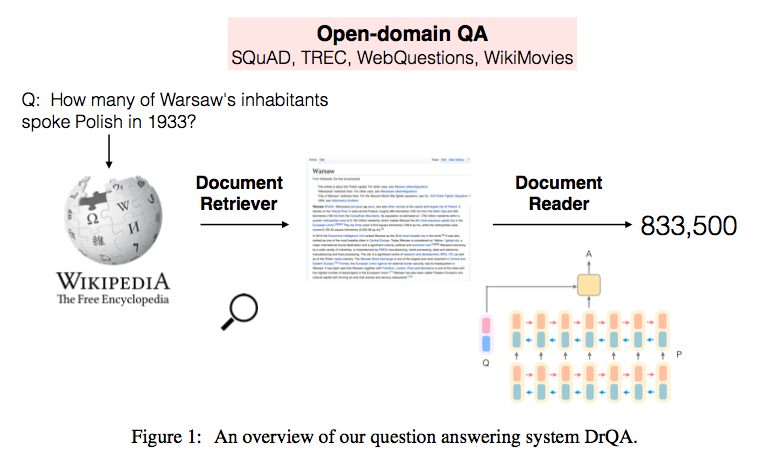
\includegraphics[width=\linewidth]{fig_QA/structure.png}
		%\caption{Structure}
		\label{fig:structure}
	\end{figure}
%=======================================
\subsection{Document Retriever}
	The Document Retriever is quite simple, it use the technique of TF-IDF\citep{salton1988term} to scoring the articles in the database and the question, then get the most similar documents to the specific question.  \par
\subsubsection{TF-IDF}
	TF, short for term frequency, is the number of times that a term occurs in the article. \par
	\begin{equation}
		TF(t, document)=\frac{Number\ of\ times\ term\ t\ appears\ in\ the\ document}{Number\ of\ terms\ in\ the\ document}
	\end{equation} \par
	IDF, short for inverse document frequency, which measures the amount of information of the term provides, that means, whether the term is common or rare across all documents. \par
	\begin{equation}
		IDF(t)=log(\frac{Number\ of\ documents}{Number\ of\ documents\ term\ t\ has\ appeared\ in})
	\end{equation} \par
	TF-IDF is the product of TF and IDF:
	\begin{equation}
		\text{TF-IDF}(t, document) = TF(t, document) \cdot IDF(t)
	\end{equation} \par
	As an example, in the documents here:
	\begin{figure}[H]
		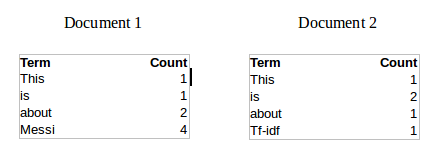
\includegraphics[width=\linewidth]{fig_QA/tfidf.png}
		%\caption{Structure}
		\label{fig:tfidf}
	\end{figure} \par
	We can calculate the TF and IDF seperately:
	\begin{align*}
		TF("This",Document1) &= \frac{1}{8} \\
		TF("This",Document2) &= \frac{1}{5} \\
		TF("Messi",Document1) &= \frac{4}{8} 
	\end{align*} \par
	\begin{align*}
		IDF("This") &= log(\frac{2}{2}) = 0 \\
		IDF("Messi") &= log(\frac{2}{1}) = 0.301
	\end{align*} \par
	And then get the TF-IDF:
	\begin{align*}
		\text{TF-IDF}("This",Document1) &= \frac{1}{8} * 0 = 0\\
		\text{TF-IDF}(("This",Document2) &= \frac{1}{5} *0 = 0\\
		\text{TF-IDF}(("Messi",Document1) &= \frac{4}{8} * 0.301 = 0.15
	\end{align*} \par	
	As you can see for Document1 , TF-IDF method heavily penalizes the word "This" but assigns greater weight to "Messi". So, this may be understood as "Messi" is an important word for Document1 from the context of the entire corpus. \par
	Here we used TF-IDF to calculate the similarity of the question and documents like this:
	\begin{enumerate}
	\item Calculate the TF-IDF of each word in the question.
	\item Calculate the TF-IDF of the words in the documents.
	\item Dot product between the TF-IDF weighted word vector spaces of question and documents.
	\item Choose the documents with the highest values calculated above.
	\end{enumerate}
%=======================================
\subsection{Document Reader}
\subsubsection{Word Embedding}
	Each word in the articles and the questions should be represented in vectors. Here, we use pre-trained word vectors GloVe\citep{pennington2014glove} to obtain the fixed word embedding of each word. 
	\begin{figure}[H]
		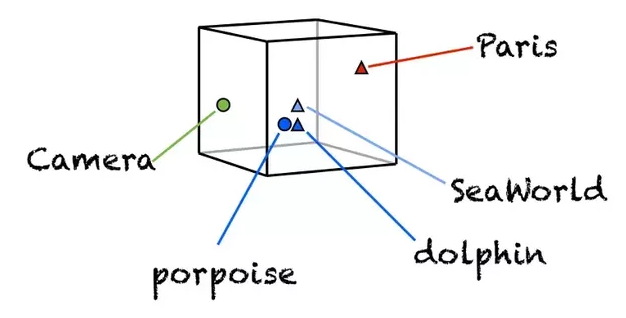
\includegraphics[width=\linewidth]{fig_QA/wordembedding.png}
		%\caption{Structure}
		\label{fig:wordembedding}
	\end{figure} \par
\subsubsection{Recurrent Neural Network(RNN)}
	The Recurrent Neural Network(RNN)\citep{Goodfellow-et-al-2016-Book} is a generalization of feedforward neural networks to sequences. And for this task of Reading Comprehension, the inputs are sequences, so fit for the RNNs. \par
%------------------------------------------------------------------
\subsubsection{Bidirectional RNNs}
	The correct interpretation of the current token is not simply depend on the the former tokens but also the tokens after. Bidirectional RNNs were invented to fulfill this kind of requirement\citep{Goodfellow-et-al-2016-Book}. \par
%------------------------------------------------------------------
\subsubsection{Long Short-Term Memory(LSTM)}
	The RNNs have a difficulty called long-term dependencies. In RNNs, they apply the same operation at each time step of a long temporal sequence repeatedly. That cause the gradient easy to vanish or explode. \par
	To solve this problem, that means to let the gradient flow for long durations, one network called long short-term memory(LSTM) is introduced\citep{hochreiter1997long} and used here.
%------------------------------------------------------------------
\subsubsection{Attention Mechanisms}
	Attention model is to introduce a focus on a specific parts of the input sequences, which was first applied in NLP by Bahdanau et al.\citep{bahdanau2014neural} on \textbf{Neural Machine Translation}. Last year, Yin et al.\citep{yin2016simple} tackled \textbf{simple question answering} by an attentive convolutional neural network. And here also applied the attention model.\par
	An aligned question embedding is:
	\begin{equation}
		f_{align}(p_i)=\sum_i a_{i,j}\bm{E}(q_j)
	\end{equation}
where, $\bm{E}(q_j)$ is the word embedding vector of token $q_j$, and:
	\begin{equation}
		a_{i,j}=\frac{exp(\alpha(\bm{E}(p_i))\cdot\alpha(\bm{E}(q_j)))}{\sum_{j'}exp(\alpha(\bm{E}(p_i))\cdot\alpha(\bm{E}(q_{j'})))}
	\end{equation}
which captures the similarity between $p_i$ and each question words $q_j$. \par
%------------------------------------------------------------------
\subsubsection{Paragraph encoding}
	Paragraph encoding used a multi-layer bidirectional LSTM over the feature vector $\widetilde{\bm{p}}_i$: \par
	\begin{equation}
		\{\bm{p_1,...,p_m}\}=RNN(\{\widetilde{\bm{p}}_1,...,\widetilde{\bm{p}}_m \})
	\end{equation}	
	The $\widetilde{\bm{p}}_i$ is comprised of four parts:
	\begin{itemize}
		\item Word embeddings
		\item Exact match
		\item Token features
		\item Aligned question embedding
	\end{itemize}
%------------------------------------------------------------------
\subsubsection{Question encoding}
	Question encoding used another LSTM over the word embeddings of $q_i$ and combine it into one single vector:
	\begin{equation}
		\bm{q}=\sum_j b_j\bm{q_j}
	\end{equation}	
where,
	\begin{equation}
		b_j = \frac{exp(\bm{w}\cdot\bm{q_j)}}{\sum_{j'}exp(\bm{w}\cdot\bm{q_j')}}
	\end{equation}
$\bm{w}$ is a weight vector to learn. \par
%------------------------------------------------------------------
\subsubsection{Prediction}
	The input of the prediction is $\{\bm{p_1,...,p_m}\}$ and $\bm{q}$. \par
	The goal is to predict the span of tokens that is most likely the correct answer by:
	\begin{equation}
		i,j=argmax_{i,i \le j \le i+15} exp(\bm{p_iW_sq})exp(\bm{p_{j}W_eq})
	\end{equation}	
	This is the object function. We use the dataset to train on this function to get the highest possible answers.
%=======================================
\subsection{Data Source}
	The knowledge source is Wikipedia. This is used for document retriever.\par
	To train Document Reader, used SQuAD. \par
	To test the QA system, used SQuAD, CuratedTREC, WebQuestions and WikiMovies. \par
%=======================================
\section{Results}
The results are quite good for three of the datasets, but one is not that good. As shown below:
	\begin{figure}[H]
		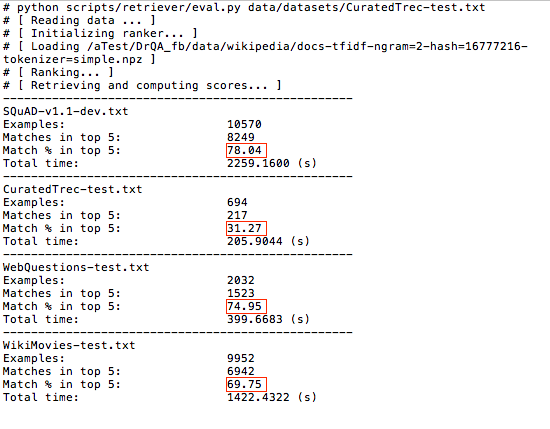
\includegraphics[width=\linewidth]{fig_QA/results.png}
		%\caption{Structure}
		\label{fig:results}
	\end{figure} \par
\section{Demonstration}	
We try the question: "What is Artificial Intelligence?" It gave the following answer:
	\begin{figure}[H]
		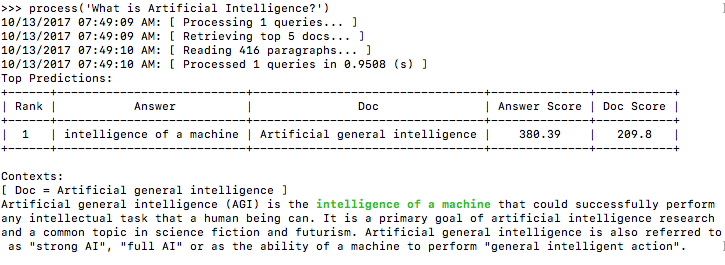
\includegraphics[width=\linewidth]{fig_QA/demo.png}
		%\caption{Structure}
		\label{fig:demo}
	\end{figure} \par
Another question:"who is Napoleon Bonaparte?":
	\begin{figure}[H]
		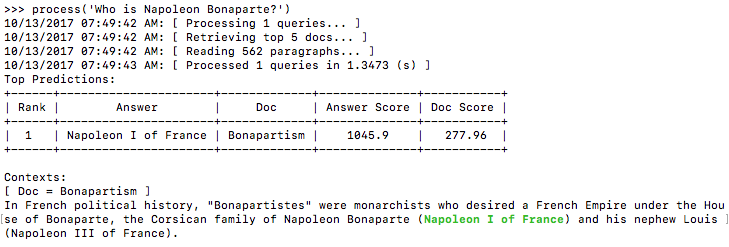
\includegraphics[width=\linewidth]{fig_QA/demo2.png}
		%\caption{Structure}
		\label{fig:demo2}
	\end{figure} \par
For non-factoid questions, it could not gave a quite meaningful answer:
	\begin{figure}[H]
		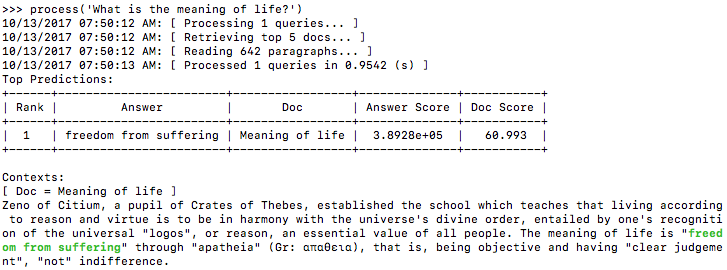
\includegraphics[width=\linewidth]{fig_QA/demo3.png}
		%\caption{Structure}
		\label{fig:demo3}
	\end{figure} \par
So this system is for factoid question-answering, and for non-factoid question-answering, it is not that good for that. \par
%=======================================
\section{Potential Improvements}
There are also lots of improvements that can be done, but we still not have time to implement them. \par
The following are some of the potential improvements:
	\begin{itemize}
		\item Data Source of the document retriever \par
		The data source here is just Wikipedia, but it could be the whole web sites, using the search engine(google for example).
		\item Data source of the document reader \par
		Use other emerging data sources(for example, the new dataset MS MACRO\citep{nguyen2016ms}).
		\item Document Retriever \par
		Document retriever is a kind of information retrieval, so we could use some more sophisticated Information retrieval techniques.
		\item Document Reader \par
		Document reader is a task of Reading Comprehension, and there are lots of papers focused on this task, so we could use some other structures improved recently.
		\item Ensemble of models \par
		Lots of results were improved by ensemble of models. So we could try to applicate several models instead of just one.
	\end{itemize}
%=======================================
\renewcommand\refname{Reference}
\bibliographystyle{unsrtnat}
\bibliography{QA}
\clearpage
\end{document}